\section{Basic Notions}
    \begin{ldefinition}{Sets}{Sets}
        A \gls{set} is a collection of objects, called elements, none of which
        is the set itself. Given a set $A$ and an element $x$, we denote that
        $x$ is contained in $A$ by writing $x\in{A}$. If $x$ is not an
        element of $A$, we write $x\notin{A}$.
    \end{ldefinition}
    The notion of a \textrm{set} is often left undefined, and we haven't
    defined it very well here, either. The terms \textit{collection} and
    \textit{object} have not been defined, and thus this definition is
    somewhat meaningless. Intuitively, a set is a bunch of things that we can
    discuss, either by the properties these things have, or by listing them
    out.
    \begin{lexample}{Basic Sets}{Example_of_Basic_Sets}
        When possible it is convenient to simply list out the elements of a
        set. The standard notation is to enclose the elements in braces,
        separated by commas.
        \begin{equation}
            A=\{\,1,\,2,\,3\,\}
        \end{equation}
        Here, $A$ is a set and it is entirely determined by the elements 1, 2,
        and 3. Sets need not only be concerned with numbers, and we can allow
        for abstract objects.
        \par
        \begin{subequations}
            \begin{minipage}[b]{0.49\textwidth}
                \centering
                \begin{equation}
                    B=\{\,a,\,b,\,c\,\}
                \end{equation}
            \end{minipage}
            \hfill
            \begin{minipage}[b]{0.49\textwidth}
                \centering
                \begin{equation}
                    C=\{\,\textrm{Boston, New York}\,\}
                \end{equation}
            \end{minipage}
        \end{subequations}
        \par\vspace{2.5ex}
        Both of these are valid sets.
    \end{lexample}
    \begin{lexample}{}{Sets_with_Ellipses}
        The examples described in Ex.~\ref{ex:Example_of_Basic_Sets} are all
        finite and contain a small number of elements. For larger sets we use
        ellipses to indicate some pattern. For example:
        \par
        \begin{subequations}
            \begin{minipage}[b]{0.49\textwidth}
                \centering
                \begin{align}
                    \mathbb{Z}_{3}&=\{\,1,\,2,\,3\,\}\\
                    \mathbb{Z}_{4}&=\{\,1,\,2,\,3,\,4\,\}
                \end{align}
            \end{minipage}
            \hfill
            \begin{minipage}[b]{0.49\textwidth}
                \centering
                \begin{align}
                    \mathbb{Z}_{6}  &=\{\,1,\,2,\,\dots,\,5,\,6\,\}\\
                    \mathbb{Z}_{108}&=\{\,1,\,2,\,\dots,\,107,\,108\,\}
                \end{align}
            \end{minipage}
        \end{subequations}
        \par\vspace{2.5ex}
        For infinite sets it is best to use what is known as
        \textit{Set-Builder} notation, but when a pattern is clear enough
        ellipses can suffice. The set of natural numbers and the set of
        integers are often described this way:
        \begin{subequations}
            \begin{align}
                \label{eqn:Natural_Numbers_Ellipses}%
                \mathbb{N}&=\{\,1,\,2,\,3,\,\dots\,\}\\
                \label{eqn:Integers_Ellipses}%
                \mathbb{Z}&=\{\,\dots,\,\minus{3},\,\minus{2},\,\minus{1},\,
                                0,\,1,\,2,\,3,\,\dots\,\}
            \end{align}
        \end{subequations}
        Rigorous definitions for both of these sets will be given after we've
        developed set theory more thoroughly.
    \end{lexample}
    The requirement that a set cannot contain itself is to avoid various
    paradoxes, such as the one discovered by Bertrand Russell in 1901. To
    avoid such problems, Ernst Zermello proposed a collection of
    \textit{axioms} in 1908. Subtle problems were pointed out by Abraham
    Fraenkel in 1921, and eventually the system known as Zermelo-Fraenkel
    Set Theory came to be. The condition that a set cannot contain itself can
    be restated as the \textit{Axiom of Regularity}. It is phrased as follows:
    \begin{axiom}[Axiom of Regularity]
        \label{ax:Axiom_of_Regularity}%
        If $A$ is a non-empty set, then there is a set $B\in{A}$
        such that that $A$ and $B$ are disjoint.
    \end{axiom}
    We've yet to discuss what empty and non-empty means, nor have we discussed
    the definition of disjoint. Intuitively, non-empty means the set has
    \textit{something} contained in it, and disjoint sets are sets with
    nothing in common. That is, none of their elements are the same. The axiom
    of regularity implies that, given a set $A$, it is impossible for $A$
    to be an element of $A$.
    \begin{axiom}[Axiom of the Empty Set]
        \label{ax:Axiom_of_the_Empty_Set}%
        There exists a set $\emptyset$ such that, if $x$ is an element,
        then $x\notin\emptyset$.
    \end{axiom}
    This axiom is used to define and justify the existence of the empty set.
    \begin{ldefinition}{The Empty Set}{Empty_Set}
        The \gls{empty set} is the set $\emptyset$ such that,
        for all $x$, it is true that $x\notin\emptyset$.
    \end{ldefinition}
    The empty set contains no elements and we occasionally write
    $\emptyset=\{\}$. It is unique. Note that the empty set is different from
    the set $\{\emptyset\}$. Indeed, this would violate our requirement that
    sets do not contain themselves. The empty set contains no elements,
    whereas $\{\emptyset\}$ contains one element (It contains the empty set).
    \subsection{Subsets}
        A set is determined entirely by it's elements. Thus repetition of
        elements cannot be accounted for, and the sets $\{a,\,b\}$ and
        $\{a,\,a,\,b\}$ must be considered the same, since they have exactly
        the same elements. Similarly, $\{a,\,b\}$ and $\{b,\,a\}$ are the
        same. To distinguish between such things requires a notion of order.
        This is achieved by introducing the notions of \textit{ordered pairs}
        and \textit{functions}. To rigorously show that the three
        aforementioned sets are indeed the same will require a definition of
        equality.
        \begin{ldefinition}{Subsets}{Subsets}
            A \gls{subset} of a set $B$ is a set $A$, denoted $A\subseteq{B}$,
            such that for all $x\in{A}$, it is true that $x\in{B}$. We write
            $A\nsubseteq{B}$ to denote that $A$ is not a subset of $B$.
        \end{ldefinition}
        We can often picture sets and subsets as blobs in the plane
        (Fig.~\ref{fig:Subset_Blobs}). In this figure, the blob $A$ is
        entirely contained within the blob $B$, and thus $A$ is a subset of
        $B$. The definition of subset allows us to rigorously define the
        notion of equality.
        \begin{figure}[H]
            \centering
            %--------------------------------Dependencies----------------------------------%
%   tikz                                                                       %
%-------------------------------Main Document----------------------------------%
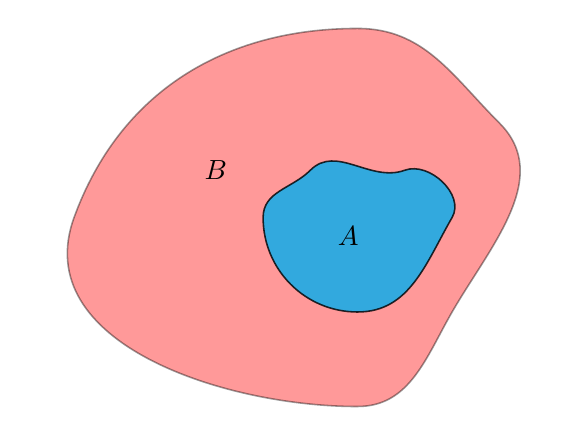
\begin{tikzpicture}[line width=0.2mm, scale=1.2]

    % Coordinates for the bigger blob.
    \coordinate (P1) at ( 0.0, -2.0);
    \coordinate (P2) at ( 1.0, -1.0);
    \coordinate (P3) at ( 1.5,  1.0);
    \coordinate (P4) at ( 0.0,  2.0);
    \coordinate (P5) at (-3.0,  0.0);

    % Coordinates for the inner blob.
    \coordinate (Q1) at ( 0.0, -1.0);
    \coordinate (Q2) at ( 1.0,  0.0);
    \coordinate (Q3) at ( 0.5,  0.5);
    \coordinate (Q4) at (-0.5,  0.5);
    \coordinate (Q5) at (-1.0,  0.0);

    % Coordindates to label things.
    \coordinate (A) at (-0.1, -0.2);
    \coordinate (B) at (-1.5,  0.5);

    % Draw the bigger blob.
    \draw[fill=red, opacity=0.4] (P1) to [out=0,    in=-120] (P2)
                                      to [out=60,   in=-45]  (P3)
                                      to [out=135,  in=0]    (P4)
                                      to [out=-180, in=70]   (P5)
                                      to [out=-110, in=-180] cycle;

    % Draw the inner blob.
    \draw[fill=cyan, opacity=0.8] (Q1) to [out=0,    in=-120]  (Q2)
                                       to [out=60,   in=20]    (Q3)
                                       to [out=-160, in=45]    (Q4)
                                       to [out=-135, in=90]    (Q5)
                                       to [out=-90,  in=180]   cycle;

    % Labels for the two blobs.
    \node at (A) {$A$};
    \node at (B) {$B$};
\end{tikzpicture}

            \caption[Visual for Subsets]
                    {Sets can be Visualized as Blobsin the Plane.}
            \label{fig:Subset_Blobs}
        \end{figure}
        \begin{lexample}{Subsets}{Basic_Subsets}
            If we let $A$ and $B$ be the sets defined by:
            \par
            \begin{subequations}
                \begin{minipage}[b]{0.49\textwidth}
                    \centering
                    \begin{equation}
                        A=\{\,1,\,2,\,3\,\}
                    \end{equation}
                \end{minipage}
                \hfill
                \begin{minipage}[b]{0.49\textwidth}
                    \centering
                    \begin{equation}
                        B=\{\,1,\,2,\,3,\,4,\,5\,\}
                    \end{equation}
                \end{minipage}
            \end{subequations}
            \par\vspace{2.5ex}
            Then we see that $A$ is a subset of $B$ since every element of
            $A$ is also an element of $B$. To express this, we write
            $A\subseteq{B}$. However, $B$ is not a subset of $A$ since the
            element 4 is contained in $B$ but it is not contained in $A$.
            Thus we may write $B\nsubseteq{A}$, indicating that $B$ is not a
            subset of $A$. Furthermore, if we define:
            \begin{equation}
                C=\{\,4,\,5,\,6,\,7,\,8\,\}
            \end{equation}
            Then we see that neither $B$ is a subset of $C$, nor is $C$ a
            subset of $B$. That is, $B\nsubseteq{C}$ and $C\nsubseteq{B}$.
            This is because $B$ has elements that aren't in $C$, and
            $C$ has elements that aren't in $B$. Moreover, $A$ and $C$ have
            zero elements in common, and are thus said to be
            \textit{disjoint}.
        \end{lexample}
        From the definition of subsets we see that for any set $A$ it is
        true that $A$ is a subset of itself. That is, $A\subseteq{A}$. It
        would be useful to distinguish between subsets that aren't the entire
        set. Such beings are called proper subsets.
        \begin{ldefinition}{Equal Sets}{Equal_Sets}
            \Glspl{equal set} are sets $A$ and $B$, denoted $A=B$, such that
            $A\subseteq{B}$ and $B\subseteq{A}$.
        \end{ldefinition}
        \begin{lexample}{Equal Sets}{Equal_Sets}
            As stated before, sets do not have a notion of order,
            nor can they account for repetition. For let $A$ and $B$
            be sets defined by:
            \par
            \begin{subequations}
                \begin{minipage}[b]{0.49\textwidth}
                    \centering
                    \begin{equation}
                        A=\{\,a,\,b\,\}
                    \end{equation}
                \end{minipage}
                \hfill
                \begin{minipage}[b]{0.49\textwidth}
                    \centering
                    \begin{equation}
                        B=\{\,a,\,a,\,b\,\}
                    \end{equation}
                \end{minipage}
            \end{subequations}
            \par\vspace{2.5ex}
            Then $A=B$. For $A\subseteq{B}$, since for all $x\in{A}$, it is
            true that $x\in{B}$. But also $B\subseteq{A}$, since if
            $x\in{B}$ then either $x=a$ or $x=b$. But $a$ and $b$ are elements
            of $A$ and thus, if $x\in{B}$, then it is true that $x\in{A}$
            and therefore $B\subseteq{A}$. By the definition of equality
            (Def.~\ref{def:Equal_Sets}), $A=B$. If we further define:
            \begin{equation}
                C=\{b,\,a\}
            \end{equation}
            Then again we see that $A=C$, since $A\subseteq{C}$ and
            $C\subseteq{A}$.
        \end{lexample}
        Zermelo-Fraenkel set theory defines equality via
        the \textit{Axiom of Extensionality}:
        \begin{axiom}[Axiom of Extensionality]
            If $A$ and $B$ are sets, and if for all $x$ it is true that
            $x\in{A}$ if and only if $x\in{B}$, then $A=B$.
        \end{axiom}
        This is precisely what we've stated, but we've used the language of
        subsets. Also, rather than stating equality as an axiom, we've
        presented it as a definition. The differences are purely semantical.
        We can now define proper subsets.
        \begin{ldefinition}{Proper Subset}{Proper_Subset}
            A \gls{proper subset} of a set $B$ is a set $A\subseteq{B}$,
            denoted $A\subsetneq{B}$, such that $A\ne{B}$.
        \end{ldefinition}
        The symbols $\subseteq$ and $\subsetneq$ are analogous to the
        notations of inequalities that one finds in calculus: $\leq$ and $<$.
        In many texts, the two symbols $\subseteq$ and $\subset$ are taken to
        be identical, which may cause confusion. In an attempt to reduce
        confusion, $\subseteq$ will denote any subset, $\subsetneq$ denotes a
        proper subset, and the symbol $\subset$ will be avoided.
        \begin{lexample}{Proper Subsets}{Proper_Subsets}
            Let $A$ and $B$ be sets defined as follows:
            \par
            \begin{subequations}
                \begin{minipage}[b]{0.49\textwidth}
                    \centering
                    \begin{equation}
                        A=\{\,a,\,b,\,c\,\}
                    \end{equation}
                \end{minipage}
                \hfill
                \begin{minipage}[b]{0.49\textwidth}
                    \centering
                    \begin{equation}
                        B=\{\,a,\,b,\,c,\,d\,\}
                    \end{equation}
                \end{minipage}
            \end{subequations}
            \par\vspace{2.5ex}
            Then $A\subseteq{B}$, since every element of $A$ is an element of
            $B$, but $B\nsubseteq{A}$ since $d\in{B}$ and $d\notin{A}$.
            Therefore $A\ne{B}$, and thus $A$ is a  proper subset of $B$.
            We denote this by writing $A\subsetneq{B}$.
        \end{lexample}
    \subsection{Ordered Pairs and Cartesian Products}
        Before we can begin stating and proving theorems, we need an
        indispensable tool: \textit{The Law of the Excluded Middle}. This
        states that, given a proposition $P$, either $P$ is true or $P$ is
        not true. It allows us to prove theorems via
        \textit{proof by contradiction}. That is, we assume the opposite and
        arrive at a contradiction, thus proving the original statement was
        true. The law of the excluded middle is a theorem, known as
        Diaconescu's Theorem, that follows from the \textit{Axiom of Choice}.
        This is a very strong, but controversial, axiom of set theory. It is
        common in analysis to adopt the axiom, and it's use is widespread in
        many theorems. To discuss the axiom of choice we first need to
        develop the notions of function and union.
        \begin{axiom}[Axiom of Pairing]
            \label{ax:Axiom_of_Pairing}%
            If $a$ and $b$ are elements, then there is a set $A$ such that
            $z\in{A}$ if and only if either $z=a$ or $z=b$. That is,
            $A=\{\,a,\,b\,\}$.
        \end{axiom}
        The axiom of pairing simply states that, given two things, we can
        form a set that is defined entirely by these two things. This is
        used to proved \textit{ordered pairs} exist.
        \begin{theorem}
            \label{thm:Existence_of_Ordered_Pair}%
            If $x$ and $y$ are elements, then there exists a set $A$ such
            that $z\in{A}$ if and only if $z=\{\,x\,\}$ or $z=\{\,x,\,y\,\}$.
        \end{theorem}
        \begin{proof}
            For let $a=x$ and $b=x$. Then, by the axiom of pairing
            (Ax.~\ref{ax:Axiom_of_Pairing}), there is a set
            $\{\,a,\,b\,\}=\{\,x,\,x\,\}$. But by the definition of equality
            (Def.~\ref{def:Equal_Sets}), $\{\,x,\,x\,\}=\{\,x\,\}$. Again, by
            the axiom of pairing, letting $a=x$ and $b=y$, we have that the
            set $\{\,x,\,y\,\}$ exists. Finally, invoking the axiom of
            pairing, and letting $a=\{\,x\,\}$ and $b=\{\,x,\,y\,\}$, we have
            that the set $\{\,\{\,x\,\},\,\{\,x,\,y\,\}\,\}$ exists.
        \end{proof}
        \begin{ldefinition}{Ordered Pair}{Ordered_Pair}
            The \gls{ordered pair} of an element $x$ with respect
            to an element $y$ is the set:
            \begin{equation}
                (x,\,y)\equiv\big\{\,\{\,x\,\},\,\{\,x,\,y\,\}\,\big\}
            \end{equation}
            Where the symbol $\equiv$ used here means ``Is defined by.''
        \end{ldefinition}
        Thm.~\ref{thm:Existence_of_Ordered_Pair} allows us to define ordered
        pairs in a manner that is consistent with ZFC. That is, if the axioms
        we are adopting are consistent, then so is our definition. Note that
        from the definition, given two distinct elements $x$ and $y$,
        $(x,\,y)\ne(y,\,x)$. This definition is due to Kazimierz Kuratowski
        and was first put forward in 1921. It does precisely what we want for
        an ordered pair, and distinguishes the order of the elements. There
        is a slight caveat, for we have the following reduction:
        \begin{equation}
            (x,\,x)=\big\{\,\{\,x\,\},\,\{\,x,\,x\,\}\,\big\}
                   =\big\{\,\{\,x\,\},\,\{\,x\,\}\,\big\}
                   =\big\{\,\{\,x\,\}\,\big\}
        \end{equation}
        This does not create too much of an issue.
        An alternative definition was put forward by Norbert Wiener in 1914:
        \begin{equation}
            (x,\,y)_{W}=\Big\{\,\big\{\{x\},\,\emptyset\big\},\,
                                \big\{\{y\}\big\}\Big\}
        \end{equation}
        Wiener used this definition since he was interested in things called
        \textit{types}. This is connected to Bertrand Russell's Type Theory,
        which was an attempt to free set theory of the paradoxes he
        discovered. Kuratowski's definition is sufficient for almost all
        purposes, and it's the one we shall adopt.
        \begin{lexample}{}{Ordered_Pair_1_2_vs_2_1}
            Consider the ordered pair $(1,\,2)$, where we take for granted
            that $1\ne{2}$. Using Kuratowski's definition
            (Def.~\ref{def:Ordered_Pair}), we obtain:
            \begin{equation}
                (1,\,2)=\big\{\,\{\,1\,\},\,\{\,1,\,2\,\}\,\big\}
            \end{equation}
            Swapping and computing $(2,\,1)$, we have:
            \begin{equation}
                (2,\,1)=\big\{\,\{\,2\,\},\,\{\,2,\,1\,\}\,\big\}
            \end{equation}
            Now the sets $\{1,\,2\}$ and $\{2,\,1\}$ are equal, since they
            contain the same elements. Therefore $\{1,\,2\}$ is an element
            of both $(1,\,2)$ and $(2,\,1)$. However $\{1\}$ is an element
            of $(1,\,2)$, and not and element of $(2,\,1)$, and thus
            $(1,\,2)\nsubseteq(2,\,1)$. Similarly, $\{2\}$ is an element of
            $(2,\,1)$, but not an element of $(1,\,2)$, and thus
            $(2,\,1)\nsubseteq(1,\,2)$. Thus, we have that
            $(1,\,2)\ne(2,\,1)$, as desired.
        \end{lexample}
        To order sets that have more than two
        elements we must first define functions. Functions are defined in
        terms of the \textit{Cartesian Product} of two sets. To do this we
        need another axiom from Zermelo-Fraenkel Set Theory: The
        \textit{Axiom Schema of Specification}. This allows us to construct
        sets via \textit{Set-Builder Notation}.
        \begin{axiom}[Axiom Schema of Specification]
            \label{ax:Axiom_Schema_of_Specification}%
            If $B$ is a set and $P$ is a proposition, then there is a set
            $A\subseteq{B}$ such that $x\in{A}$ if and only if $x\in{B}$ and
            $P(x)$ is true.
        \end{axiom}
        This axiom states that the Set-Builder method of constructing sets is
        valid. We have seen that the natural numbers $\mathbb{N}$ and the
        integers $\mathbb{Z}$ (From the German \textit{Zahl}) can be loosely
        described by using ellipses to indicate a pattern
        (Eqns.~\ref{eqn:Natural_Numbers_Ellipses}-%
        \ref{eqn:Integers_Ellipses}, respectively). It would be more
        difficult (But not impossible) to describe the set of rational
        numbers in such a way. Instead, we use set
        builder notation. We can describe the set of rational numbers
        $\mathbb{Q}$ as follows:
        \begin{equation}
            \mathbb{Q}=\Big\{\;\frac{p}{q}\in\mathbb{R}\,:
                               \,p,\,q\in\mathbb{Z}
                               \textrm{ and }q\ne{0}\;\Big\}
        \end{equation}
        That is, the rational numbers are the set of all real numbers which
        can be written as the ratios of integers with non-zero denominator.
        The Axiom Schema of Specification states that this is is a valid
        method of describing sets. It is also known as the axiom of
        separation.
        \par\hfill\par
        It is crucial to note the requirement that the set we our building
        with our proposition is a subset of some larger set. For
        $\mathbb{Q}$ we assumed there exists some set $\mathbb{R}$ (The
        real numbers). The axiom does not allow us to simply write
        \textit{The set of all $x$ such that $P(x)$ is true}. Indeed, this is
        precisely how one arrives at Russell's paradox. The axiom
        allows us to write
        \textit{The set of all $x$ such that $x\in{B}$ and $P(x)$ is true},
        where $B$ is some set whose existence has already been established.
        \begin{lexample}{Set-Builder Notation}{Set_Builder_Evens_and_Odds}
            Again supposing that the natural numbers have been defined for us,
            we can use this to construct other sets. An even natural number
            is an integer $n\in\mathbb{N}$ such that $n/2$ is also an integer.
            Similarly, an odd natural number is a an integer $n\in\mathbb{N}$
            such that $n$ is not even. We can describe the sets of even and
            odd numbers via ellipses, and we write:
            \par
            \begin{subequations}
                \begin{minipage}[b]{0.49\textwidth}
                    \centering
                    \begin{equation}
                        \mathbb{N}_{e}=\{\,2,\,4,\,6,\,8,\,\dots\,\}
                    \end{equation}
                \end{minipage}
                \hfill
                \begin{minipage}[b]{0.49\textwidth}
                    \centering
                    \begin{equation}
                        \mathbb{N}_{o}=\{\,1,\,3,\,5,\,7,\,\dots\,\}
                    \end{equation}
                \end{minipage}
            \end{subequations}
            \par\vspace{2.5ex}
            But rather than doing this, we can introduce rigor and describe
            these sets using Set-Builder notation. We write:
            \par
            \begin{subequations}
                \begin{minipage}[b]{0.49\textwidth}
                    \centering
                    \begin{equation}
                        \mathbb{N}_{e}=\{\;n\in\mathbb{N}:
                                           n\textrm{ is even.}\;\}
                    \end{equation}
                \end{minipage}
                \hfill
                \begin{minipage}[b]{0.49\textwidth}
                    \centering
                    \begin{equation}
                        \mathbb{N}_{o}=\{\;n\in\mathbb{N}:
                                           n\textrm{ is odd.}\;\}
                    \end{equation}
                \end{minipage}
            \end{subequations}
            \par\vspace{2.5ex}
            Such notation is justified by the axiom schema of specification.
        \end{lexample}
        Next, we discuss the \textit{axiom of union}.
        \begin{axiom}[Axiom of Union]
            \label{ax:Axiom_of_Union}%
            If $\mathcal{O}$ is a set, then there is a set $A$ such that, for
            all $x$, $x\in{A}$ if and only if there is an $F\in\mathcal{O}$
            such that $x\in{F}$.
        \end{axiom}
        This states that given a collection of sets, we can form a new sets
        whose elements are the elements of the sets in our collection. This
        is best illustrated by example.
        \begin{lexample}{Axiom of Union}{Axiom_of_Union}
            Let $A$ and $B$ be sets defined as follows:
            \par
            \begin{subequations}
                \begin{minipage}[b]{0.49\textwidth}
                    \centering
                    \begin{equation}
                        A=\{\,1,\,2,\,3\,\}
                    \end{equation}
                \end{minipage}
                \hfill
                \begin{minipage}[b]{0.49\textwidth}
                    \centering
                    \begin{equation}
                        B=\{\,2,\,3,\,4\,\}
                    \end{equation}
                \end{minipage}
            \end{subequations}
            \par
            \vspace{2.5ex}
            Using the axiom of pairing, we can create the following set:
            \begin{equation}
                \mathcal{O}=\{\,A,\,B\,\}
            \end{equation}
            The axiom of union says that we can form a new set $C$ defined as
            the set of all elements contained in either $A$ or $B$:
            \begin{equation}
                C=\{\,1,\,2,\,3,\,4\,\}
            \end{equation}
            This construction, which combines the axiom of pairing and the
            axiom of union, can be used to define the union of two sets. And
            indeed, the axiom of union can be used to define union of
            arbitrarily many sets.
        \end{lexample}
        \begin{theorem}
            \label{thm:Union_of_Sets_Exists}%
            If $A$ and $B$ are sets, then there is a set $C$ such that, for
            all $x$, $x\in{C}$ if and only if $x\in{A}$ or $x\in{B}$, or both.
        \end{theorem}
        \begin{proof}
            For by the axiom of pairing (Ax.~\ref{ax:Axiom_of_Pairing}), if
            $A$ and $B$ are sets then there is a set $\mathcal{O}$ such
            that $\mathcal{O}=\{\,A,\,B\,\}$. But then by the axiom of union
            (Ax.~\ref{ax:Axiom_of_Union}) there is a set $C$ such that, for
            all $x$, $x\in{C}$ if and only if there is a set $F\in\mathcal{O}$
            such that $x\in{F}$. But then $x\in{C}$ if and only if either
            $x\in{A}$ or $x\in{B}$, or both.
        \end{proof}
        \begin{fdefinition}{Union of Two Sets}{Union_of_Two}
            The \gls{union of two sets}, $A$ and $B$, is the set
            $A\cup{B}$ define by:
            \begin{equation}
                A\cup{B}=\{\;x\,:\,x\in{A}\textrm{ or }x\in{B}\;\}
            \end{equation}
        \end{fdefinition}
        Thm.~\ref{thm:Union_of_Sets_Exists} justifies
        Def.~\ref{def:Union_of_Two}. Unions can be visualized by the use of
        Venn Diagrams (Fig.~\ref{fig:Venn_Diagram_Union}). The union of two
        sets is a commonly used construction in all branches of mathematics.
        Various theorems about it will be proved when we delve more into the
        various set operations, but we still need the law of the excluded
        middle to prove these. The last stepping stone is the axiom of the
        power set, which allows us to justify these various constructions.
        \begin{figure}[H]
            \centering
            %--------------------------------Dependencies----------------------------------%
%   tikz                                                                       %
%-------------------------------Main Document----------------------------------%
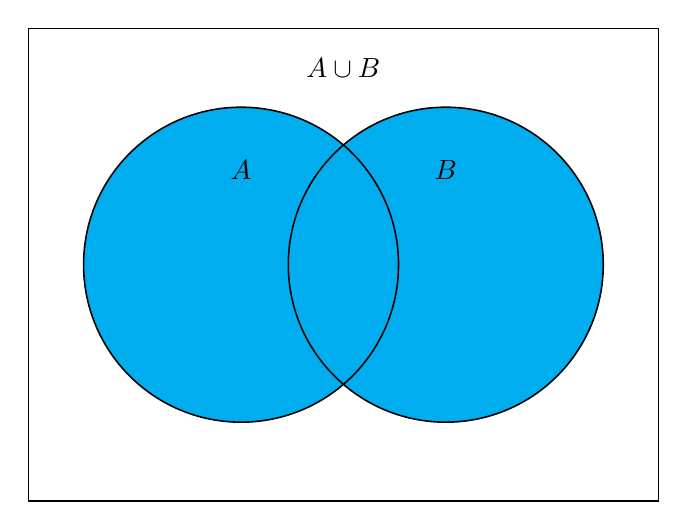
\begin{tikzpicture}[line width=0.2mm]

    % Coordinates for the centers of the circles.
    \coordinate (C1) at (-1.3, 0);
    \coordinate (C2) at ( 1.3, 0);

    % Coordinates for the labels.
    \coordinate (A) at (-1.3, 1.2);
    \coordinate (B) at ( 1.3, 1.2);
    \coordinate (U) at ( 0.0, 2.5);

    % Rectangle indicating the universe set.
    \draw (-4, -3) rectangle (4, 3);

    % Fill in the circle with cyan.
    \draw[fill=cyan, draw=none] (C1) circle (2);
    \draw[fill=cyan, draw=none] (C2) circle (2);

    % Give outlines to the circles.
    \draw (C1) circle (2);
    \draw (C2) circle (2);

    % Labels.
    \node at (A) {$A$};
    \node at (B) {$B$};
    \node at (U) {$A\cup{B}$};
\end{tikzpicture}
            \caption{Venn Diagram for Unions}
            \label{fig:Venn_Diagram_Union}
        \end{figure}
        \begin{lexample}{Union of Two Sets}{Union_of_Two_Sets}
            If we let $A$ and $B$ be defined as follows:
            \par
            \begin{subequations}
                \begin{minipage}[b]{0.49\textwidth}
                    \centering
                    \begin{equation}
                        A=\{\,3,\,5,\,6\,\}
                    \end{equation}
                \end{minipage}
                \hfill
                \begin{minipage}[b]{0.49\textwidth}
                    \centering
                    \begin{equation}
                        B=\{\,2,\,9,\,11,\,5\,\}
                    \end{equation}
                \end{minipage}
            \end{subequations}
            \par\vspace{2.5ex}
            We can form the union $A\cup{B}$ as follows:
            \begin{equation}
                A\cup{B}=\{\,2,\,3,\,5,\,6,\,9,\,11\,\}
            \end{equation}
            That is, the set of all elements in either $A$ or $B$, or both.
            We can do this construction with infinite sets as well:
            \par
            \begin{subequations}
                \begin{minipage}[b]{0.30\textwidth}
                    \centering
                    \begin{equation}
                        \mathbb{N}\cup\mathbb{Z}=\mathbb{Z}
                    \end{equation}
                \end{minipage}
                \hspace{0.03\textwidth}
                \begin{minipage}[b]{0.30\textwidth}
                    \centering
                    \begin{equation}
                        \mathbb{N}_{e}\cup\mathbb{N}_{o}=\mathbb{N}
                    \end{equation}
                \end{minipage}
                \hspace{0.03\textwidth}
                \begin{minipage}[b]{0.30\textwidth}
                    \centering
                    \begin{equation}
                        \mathbb{Q}\cup\mathbb{Z}=\mathbb{Q}
                    \end{equation}
                \end{minipage}
            \end{subequations}
            \par\vspace{2.5ex}
            Where $\mathbb{N}_{e}$, $\mathbb{N}_{o}$, $\mathbb{N}$,
            $\mathbb{Z}$, and $\mathbb{Q}$ denote the sets of even numbers,
            odd numbers, natural numbers, integers, and rational numbers,
            respectively,
        \end{lexample}
        \begin{axiom}[Axiom of the Power Set]
            \label{ax:Axiom_of_the_Power_Set}%
            If $A$ is a set, then there is a set $\mathcal{P}(A)$, called the
            power set, such that $x\in\mathcal{P}(A)$ if and only if
            $x\subseteq{A}$.
        \end{axiom}
        This axiom allows us to define the power set of any set.
        \begin{ldefinition}{Power Set}{Power_Set}
            The power set of a set $A$ is the set
            $\mathcal{P}(A)$ defined by:
            \begin{equation}
                \mathcal{P}(A)=\{\,B\,:\,B\subseteq{A}\,\}
            \end{equation}
            That is, $\mathcal{P}(A)$ is the set of all subsets of $A$.
        \end{ldefinition}
        \begin{theorem}
            \label{thm:Cartesian_Product_Exists}%
            If $A$ and $B$ are sets, then there is a set $C$ such that, for
            all $z$, $z\in{C}$ if and only if there exists $x\in{A}$ and
            $y\in{B}$ such that $z=(x,\,y)$.
        \end{theorem}
        \begin{proof}
            For let $\mathcal{O}=A\cup{B}$. Then by the axiom of the power set
            (Ax.~\ref{ax:Axiom_of_the_Power_Set}), the power set
            $\mathcal{P}(\mathcal{O})$ exists. But, again by the axiom of the
            power set, the power set
            $\mathcal{P}\big(\mathcal{P}(\mathcal{O})\big)$ exists. But then
            $z\in\mathcal{P}\big(\mathcal{P}(\mathcal{O})\big)$
            if and only if $z\subseteq\mathcal{P}(\mathcal{O})$, and for all
            $x\in{A}$ and $y\in{B}$,
            $(x,\,y)\subseteq\mathcal{P}(\mathcal{O})$. Let $P$ be the
            proposition $P(z)$ is true if and only if there exists $x\in{A}$
            and $y\in{B}$ such that $z=(x,\,y)$. Then, by the axiom schema of
            specification (Ax.~\ref{ax:Axiom_Schema_of_Specification}),
            there is a set $C$ such that:
            \begin{equation}
                C=\{\,z\,:\,P(z)\,\}
            \end{equation}
            Therefore, etc.
        \end{proof}
        The set $C$ constructed in Thm.~\ref{thm:Cartesian_Product_Exists} is
        the set of all ordered pairs of elements whose first entry is from the
        set $A$ and whose second entry comes from the set $B$. This is
        precisely the what we want the Cartesian product of $A$ with $B$ to
        be. Thus, this theorem gives justification to the following
        definition:
        \begin{ldefinition}{Cartesian Product}{Cartesian_Product}
            The \gls{Cartesian product} of a set $A$ with respect to a set
            $B$ is the set:
            \begin{equation}
                A\times{B}\equiv\{\;(a,\,b)\,:\,a\in{A}
                                    \textrm{ and }b\in{B}\;\}
            \end{equation}
            Where $(a,\,b)$ denotes the ordered pair of $a$ with $b$.
        \end{ldefinition}
        Much the way ordered pairs place order onto two arbitrary elements,
        Cartesian products place order on sets. Given two distinct sets $A$
        and $B$, we have that $A\times{B}\ne{B}\times{A}$, and thus the
        order in which we performed the Cartesian product is important. The
        validity of this statement stems from the fact that, in general,
        $(a,\,b)\ne(b,\,a)$, and thus if $A$ and $B$ are distinct sets they'll
        have at least some different elements, meaning $A\times{B}$ will have
        different ordered pairs than $B\times{A}$.
        \begin{lexample}{Cartesian Products}{Basic_Cartesian_Products}
            Let $A$ and $B$ be sets defined as follows:
            \par
            \begin{subequations}
                \begin{minipage}[b]{0.49\textwidth}
                    \centering
                    \begin{equation}
                        A=\{\,1,\,2,\,3\,\}
                    \end{equation}
                \end{minipage}
                \hfill
                \begin{minipage}[b]{0.49\textwidth}
                    \centering
                    \begin{equation}
                        B=\{\,a,\,b\,\}
                    \end{equation}
                \end{minipage}
            \end{subequations}
            \par\vspace{2.5ex}
            Let's compute $A\times{B}$ and $B\times{A}$. From the definition
            (Def.~\ref{def:Cartesian_Product}) we have:
            \begin{equation}
                A\times{B}=\{\;(a,b)\,:\,a\in{A}\textrm{ and }b\in{B}\;\}
            \end{equation}
            Using this, we can compute:
            \begin{equation}
                A\times{B}=\big\{\,(1,a),\,(2,a),\,(3,a),\,
                                   (1,b),\,(2,b),\,(3,b)\,\big\}
            \end{equation}
            Computing $B\times{A}$, we have:
            \begin{equation}
                B\times{A}=\big\{\,(a,\,1),\,(a,\,2),\,(a,\,3),\,
                                   (b,\,1),\,(b,\,2),\,(b,\,3)\,\big\}
            \end{equation}
            Now if we suppose that $a$ is not equal to 1, then we see that
            $(a,1)$ is a different element than $(1,a)$, and thus $A\times{B}$
            is not equal to $B\times{A}$. Next, compute $A\times{A}$:
            \begin{equation}
                A\times{A}=\big\{\,(1,1),\,(1,2),\,(1,3),\,
                                   (2,1),\,(2,2),\,(2,3),\,
                                   (3,1),\,(3,2),\,(3,3)\,\big\}
            \end{equation}
            And finally $B\times{B}$:
            \begin{equation}
                B\times{B}=\big\{\,(a,\,a),\,(a,\,b),
                                 \,(b,\,a),\,(b,\,b)\,\big\}
            \end{equation}
            Equality of $A\times{B}$ and $B\times{A}$ is achieved if and only
            if $A=B$, or if either set is the empty set.
        \end{lexample}
        Note that in Ex.~\ref{ex:Basic_Cartesian_Products}, the \textit{size}
        of the Cartesian product of two sets was simply the product of the
        number of elements of the constituent sets. That is, we see that $A$
        has three elements and $B$ has two elements, but also that
        $A\times{B}$ has six elements. Moreover, $A\times{A}$ has nine
        elements and $B\times{B}$ has four. This pattern holds for the
        Cartesian products of any two \textit{finite} sets.
        \par\hfill\par
        It is common to consider the Cartesian product of a set with itself.
        That is, given a set $A$, we are often interested in $A\times{A}$. We
        denote this by writing $A^{2}$. One such example is when we consider
        the set of real numbers, $\mathbb{R}$. The Cartesian product
        $\mathbb{R}^{2}$ is called the \textit{Euclidean Plane},
        or the \textit{Cartesian Plane}, after Euclid of Alexandria and
        Ren\'{e} Descartes. This is because $\mathbb{R}^{2}$ is used to model
        both planar geometry and analytical geometry, of which Euclid and
        Descartes were pioneers of, respectively. The term Cartesian products
        is in honor of Ren\'{e} Descartes, as well.
        \begin{lexample}{Plane Lattice}{Lattice_N_times_N}
            Consider $\mathbb{N}^{2}$, where $\mathbb{N}$ denotes the set of
            natural numbers (Eqn.~\ref{eqn:Natural_Numbers_Ellipses}), and
            $\mathbb{N}^{2}$ denotes the Cartesian product of this set with
            itself. We can visualize this by drawing a lattice of points in the
            plane (Fig.~\subref{fig:Lattice_Cart_Prod_of_N_with_N}).
        \end{lexample}
        \begin{lexample}{Cartesian Plane}{The_Plane_R_times_R}
            Let $\mathbb{R}$ denote the set of real numbers, and let
            $A=\mathbb{R}$ and $B=\mathbb{R}$. Then we have:
            \begin{equation}
                A\times{B}=\mathbb{R}\times\mathbb{R}\equiv\mathbb{R}^{2}
            \end{equation}
            Where the symbol $\equiv$ again means that $\mathbb{R}^{2}$ is
            defined by this expression. Using the definition of Cartesian
            products (Def.~\ref{def:Cartesian_Product}), we obtain:
            \begin{equation}
                \mathbb{R}^{2}=\{\;(x,y)\,:\,x\in\mathbb{R}
                                   \textrm{ and }y\in\mathbb{R}\;\}
            \end{equation}
            That is, $\mathbb{R}^{2}$ is the set of all ordered pairs of real
            numbers. The first term is called the $x$ coordinate, and
            similarly the second term is called the $y$ coordinate. This is
            used to model planar geometry (Fig.\subref{fig:Cartesian_Plane}).
        \end{lexample}
        \begin{figure}[H]
            \centering
            \begin{subfigure}[b]{0.49\textwidth}
                \centering
                \resizebox{\textwidth}{!}{
                    %--------------------------------Dependencies----------------------------------%
%   amssymb                                                                    %
%   tikz                                                                       %
%       arrows.meta                                                            %
%-------------------------------Main Document----------------------------------%
\begin{tikzpicture}[%
    >=Latex,
    line width=0.2mm,
    line cap=round,
    font=\Large
]
    % Coordinates for the points.
    \coordinate (x) at (2.2, 0.0);
    \coordinate (y) at (0.0, 2.9);
    \coordinate (z) at (2.2, 2.9);

    % Draw a grid.
    \draw[style=help lines] (-0.3, -0.3) grid (7.9, 7.9);

    % Axes.
    \begin{scope}[thick]
        \draw[->] (-0.3, 0) to (8.4, 0) node [above] {$\mathbb{R}$};
        \draw[->] (0, -0.3) to (0, 8.4) node [right] {$\mathbb{R}$};
    \end{scope}

    % Draw dashed lines to the point.
    \begin{scope}[densely dashed]
        \draw (x) to (z);
        \draw (y) to (z);
    \end{scope}

    % Draw dots marking the various points.
    \draw[fill=black] (x) circle (0.6mm);
    \draw[fill=black] (y) circle (0.6mm);
    \draw[fill=black] (z) circle (0.6mm);

    \node at (x) [below=0.1]     {$x$};
    \node at (y) [left=0.1]      {$y$};
    \node at (z) [above right]   {$(x,\,y)$};
\end{tikzpicture}%
                }
                \subcaption{The Cartesian Plane $\mathbb{R}^{2}$}
                \label{fig:Cartesian_Plane}
            \end{subfigure}
            \begin{subfigure}[b]{0.49\textwidth}
                \centering
                \resizebox{\textwidth}{!}{%
                    %--------------------------------Dependencies----------------------------------%
%   amssymb                                                                    %
%   tikz                                                                       %
%       arrows.meta                                                            %
%-------------------------------Main Document----------------------------------%
\begin{tikzpicture}[%
    >=Latex,
    line width=0.2mm,
    line cap=round
]

    % Axes.
    \begin{scope}[thick, font=\Large]
        \draw[->] (0, 0) to (8.4, 0) node [above] {$\mathbb{N}$};
        \draw[->] (0, 0) to (0, 8.4) node [right] {$\mathbb{N}$};
    \end{scope}

    \foreach\x in{1, 2, 3, 4, 5, 6, 7, 8}{
        \foreach\y in{1, 2, 3, 4, 5, 6, 7, 8}{
            \draw[fill=black] (\x, \y) circle (0.2mm);
        }
        \draw (\x, -0.1) to (\x, 0.1) node [below=1ex] {$\x$};
        \draw (-0.1, \x) to (0.1, \x) node [left=1ex]  {$\x$};
    }
\end{tikzpicture}%
                }
                \caption{The Lattice $\mathbb{N}^{2}$}
                \label{fig:Lattice_Cart_Prod_of_N_with_N}
            \end{subfigure}
            \caption{Examples of Cartesian Products}
            \label{fig:Cartesian_Products_Examples}
        \end{figure}
        \begin{lexample}{}{Generic_Cartesian_Product}
            Consider the following sets:
            \par
            \begin{subequations}
                \begin{minipage}[b]{0.49\textwidth}
                    \centering
                    \begin{equation}
                        A=\{\,\textrm{Point, Line 1, Line 2}\,\}
                    \end{equation}
                \end{minipage}
                \hfill
                \begin{minipage}[b]{0.49\textwidth}
                    \centering
                    \begin{equation}
                        B=\{\,\textrm{Point, Line}\,\}
                    \end{equation}
                \end{minipage}
            \end{subequations}
            \par\vspace{2.5ex}
            We can visually represent the Cartesian product $A\times{B}$ by
            drawing $A$ in green and $B$ in red, as shown in
            Fig.~\ref{fig:Cartesian_Product_Example}. The Cartesian Product
            $A\times{B}$ is the set formed by connecting all of the points
            from $A$ and $B$ in the plane. This is shown in blue.
        \end{lexample}
        \begin{figure}[H]
            \centering
            %--------------------------------Dependencies----------------------------------%
%   tikz                                                                       %
%       arrows.meta                                                            %
%-------------------------------Main Document----------------------------------%
\begin{tikzpicture}[%
    >=Latex,
    line width=0.2mm,
    line cap=round
]

    % Draw green to indicate the set A.
    \begin{scope}[green]

        % Draw some points.
        \draw[fill=green] (1, 0) circle (0.3mm);
        \draw[fill=green] (2, 0) circle (0.3mm);
        \draw[fill=green] (5, 0) circle (0.3mm);
        \draw[fill=green] (6, 0) circle (0.3mm);
        \draw[fill=green] (7, 0) circle (0.3mm);

        % Draw lines.
        \draw (2, 0) to (5, 0);
        \draw (6, 0) to (7, 0);
    \end{scope}

    % Draw red to denote the set B.
    \begin{scope}[red]

        % Draw in some points.
        \draw[fill=red] (0, 1) circle (0.3mm);
        \draw[fill=red] (0, 2) circle (0.3mm);
        \draw[fill=red] (0, 5) circle (0.3mm);

        % Draw a line.
        \draw (0, 2) to (0, 5);
    \end{scope}

    % Use blue to mark AxB (Cartesian product).
    \begin{scope}[blue]

        % Fill in points.
        \draw[fill=blue] (1, 1) circle (0.3mm);
        \draw[fill=blue] (1, 2) circle (0.3mm);
        \draw[fill=blue] (1, 5) circle (0.3mm);
        \draw[fill=blue] (2, 1) circle (0.3mm);
        \draw[fill=blue] (5, 1) circle (0.3mm);
        \draw[fill=blue] (6, 1) circle (0.3mm);
        \draw[fill=blue] (7, 1) circle (0.3mm);
        \draw[fill=blue] (2, 2) circle (0.3mm);
        \draw[fill=blue] (2, 5) circle (0.3mm);
        \draw[fill=blue] (5, 2) circle (0.3mm);
        \draw[fill=blue] (5, 5) circle (0.3mm);
        \draw[fill=blue] (6, 2) circle (0.3mm);
        \draw[fill=blue] (7, 2) circle (0.3mm);
        \draw[fill=blue] (6, 5) circle (0.3mm);
        \draw[fill=blue] (7, 5) circle (0.3mm);

        % Draw lines.
        \draw (1, 2) to (1, 5);
        \draw (2, 1) to (5, 1);
        \draw (6, 1) to (7, 1);

        % Fill in rectangles.
        \draw[fill=blue, opacity=0.4] (2, 2) to (5, 2) to (5, 5)
                                             to (2, 5) to cycle;
        \draw[fill=blue, opacity=0.4] (6, 2) to (7, 2) to (7, 5)
                                             to (6, 5) to cycle;
        \draw (2, 2) to (5, 2) to (5, 5) to (2, 5) to cycle;
        \draw (6, 2) to (7, 2) to (7, 5) to (6, 5) to cycle;
    \end{scope}
\end{tikzpicture}
            \caption[Cartesian Product of Two Sets]
                {The Cartesian Product of Two Sets. $A$ is
                 in \textcolor{green}{Green},
                 $B$ is in \textcolor{red}{red}, and
                 $A\times{B}$ is in \textcolor{blue}{blue}.}
            \label{fig:Cartesian_Product_Example}
        \end{figure}
        Cartesian products are not \textit{associative}. That is, given three
        sets $A$, $B$, and $C$, there is no clear way to take the Cartesian
        product of these since:
        \begin{equation}
            A\times(B\times{C})\ne(A\times{B})\times{C}
        \end{equation}
        To see this, note that the elements of $A\times(B\times{C})$ are
        ordered pairs of the form $\big(a,\,(b,\,c)\big)$, whereas elements of
        $(A\times{B})\times{C}$ are of the form $\big((a,\,b),\,c\big)$. When
        we write $A\times{B}\times{C}$ we really want ordered \textit{triples}
        of the form $(a,\,b,\,c)$. Much the way ordered pairs have been
        defined, we can modify Kuratowski's approach and define ordered
        triples and ordered $n$ tuples. Rather than doing this we will use the
        language of functions to define higher order Cartesian products.